\documentclass{article}\usepackage[]{graphicx}\usepackage[]{xcolor}
% maxwidth is the original width if it is less than linewidth
% otherwise use linewidth (to make sure the graphics do not exceed the margin)
\makeatletter
\def\maxwidth{ %
  \ifdim\Gin@nat@width>\linewidth
    \linewidth
  \else
    \Gin@nat@width
  \fi
}
\makeatother

\definecolor{fgcolor}{rgb}{0.345, 0.345, 0.345}
\newcommand{\hlnum}[1]{\textcolor[rgb]{0.686,0.059,0.569}{#1}}%
\newcommand{\hlsng}[1]{\textcolor[rgb]{0.192,0.494,0.8}{#1}}%
\newcommand{\hlcom}[1]{\textcolor[rgb]{0.678,0.584,0.686}{\textit{#1}}}%
\newcommand{\hlopt}[1]{\textcolor[rgb]{0,0,0}{#1}}%
\newcommand{\hldef}[1]{\textcolor[rgb]{0.345,0.345,0.345}{#1}}%
\newcommand{\hlkwa}[1]{\textcolor[rgb]{0.161,0.373,0.58}{\textbf{#1}}}%
\newcommand{\hlkwb}[1]{\textcolor[rgb]{0.69,0.353,0.396}{#1}}%
\newcommand{\hlkwc}[1]{\textcolor[rgb]{0.333,0.667,0.333}{#1}}%
\newcommand{\hlkwd}[1]{\textcolor[rgb]{0.737,0.353,0.396}{\textbf{#1}}}%
\let\hlipl\hlkwb

\usepackage{framed}
\makeatletter
\newenvironment{kframe}{%
 \def\at@end@of@kframe{}%
 \ifinner\ifhmode%
  \def\at@end@of@kframe{\end{minipage}}%
  \begin{minipage}{\columnwidth}%
 \fi\fi%
 \def\FrameCommand##1{\hskip\@totalleftmargin \hskip-\fboxsep
 \colorbox{shadecolor}{##1}\hskip-\fboxsep
     % There is no \\@totalrightmargin, so:
     \hskip-\linewidth \hskip-\@totalleftmargin \hskip\columnwidth}%
 \MakeFramed {\advance\hsize-\width
   \@totalleftmargin\z@ \linewidth\hsize
   \@setminipage}}%
 {\par\unskip\endMakeFramed%
 \at@end@of@kframe}
\makeatother

\definecolor{shadecolor}{rgb}{.97, .97, .97}
\definecolor{messagecolor}{rgb}{0, 0, 0}
\definecolor{warningcolor}{rgb}{1, 0, 1}
\definecolor{errorcolor}{rgb}{1, 0, 0}
\newenvironment{knitrout}{}{} % an empty environment to be redefined in TeX

\usepackage{alltt}
\usepackage{amsmath} %This allows me to use the align functionality.
                     %If you find yourself trying to replicate
                     %something you found online, ensure you're
                     %loading the necessary packages!
\usepackage{amsfonts}%Math font
\usepackage{graphicx}%For including graphics
\usepackage{hyperref}%For Hyperlinks
\usepackage[shortlabels]{enumitem}% For enumerated lists with labels specified
                                  % We had to run tlmgr_install("enumitem") in R
\hypersetup{colorlinks = true,citecolor=black} %set citations to have black (not green) color
\usepackage{natbib}        %For the bibliography
\setlength{\bibsep}{0pt plus 0.3ex}
\bibliographystyle{apalike}%For the bibliography
\usepackage[margin=0.50in]{geometry}
\usepackage{float}
\usepackage{multicol}

%fix for figures
\usepackage{caption}
\newenvironment{Figure}
  {\par\medskip\noindent\minipage{\linewidth}}
  {\endminipage\par\medskip}
\IfFileExists{upquote.sty}{\usepackage{upquote}}{}
\begin{document}

\vspace{-1in}
\title{Lab 7 and 8 -- MATH 240 -- Computational Statistics}

\author{
  Anya Suko\\
}

\date{27 March 2025}

\maketitle

\begin{multicols}{2}
\section{Introduction of the Beta Distribution}
%.   what is beta dist?
%.   what does it look like?
%.   what is it used for?
%.   what are its properties?
%.   what additional info do you gain from the simulations and real data analysis?

The Beta distribution is a continuous distribution, often used to model a random variable X that ranges from 0 to 1, making it useful for modeling proportions, probabilities, and rates. It is known for being remarkably flexible with regards to its shape- it can be symmetric or left/right skewed, depending on its parameters that define its shape: $\alpha > 0$, and $\beta > 0$.
 

\section{Density Function and Parameters}
The beta distribution's probablilty density function, which gives the likeliness that a continuous random variable takes on a specific value, is given by

% put function here
\[
f_x(x | \alpha, \beta) = \frac{\Gamma(\alpha + \beta)}{\Gamma(\alpha)\Gamma(\beta)}
x^{\alpha-1}(1-x)^{\beta -1} \mathbb{I}(x \in [0,1])
\]

where the density is zero anywhere outside of the range [0,1]. Since the distribution is directly impacted by its parameters ($\alpha$ and $\beta$), the population level characteristics are also described by those parameters. 

A series of example distributions were created with different $\alpha$ and $\beta$ values in order to demonstrate the effect that both $\alpha$ and $\beta$ have on the distribution, and therefore the population level characteristics.


When $\alpha$ and $\beta$ were set to 2 and 5, respectively,the population level statistics were the following:
\begin{table}[H]
\centering
\small
\begin{tabular}{|c|l|r|}
  \hline
 & Statistic & Value \\ 
  \hline
  1 & Mean & 0.29 \\ 
  2 & Variance & 0.03 \\ 
  3 & Skewness & 0.60 \\ 
  4 & Kurtosis & -0.12 \\ 
   \hline
\end{tabular}
\end{table}

When $\alpha$ and $\beta$ were set to 5 and 5, respectively,the population level statistics were the following:
\begin{table}[H]
\centering
\small
\begin{tabular}{|c|l|r|}
  \hline
 & Statistic & Value \\ 
  \hline
  1 & Mean & 0.50 \\ 
  2 & Variance & 0.02 \\ 
  3 & Skewness & 0.00 \\ 
  4 & Kurtosis & -0.46 \\ 
   \hline
\end{tabular}
\end{table}

When $\alpha$ and $\beta$ were set to 5 and 2, respectively,the population level statistics were the following:
\begin{table}[H]
\centering
\small
\begin{tabular}{|c|l|r|}
  \hline
 & Statistic & Value \\ 
  \hline
  1 & Mean & 0.71 \\ 
  2 & Variance & 0.03 \\ 
  3 & Skewness & -0.60 \\ 
  4 & Kurtosis & -0.12 \\ 
   \hline
\end{tabular}
\end{table}

When $\alpha$ and $\beta$ were set to .5 and .5, respectively,the population level statistics were the following:
\begin{table}[H]
\centering
\small
\begin{tabular}{|c|l|r|}
  \hline
 & Statistic & Value \\ 
  \hline
  1 & Mean & 0.50 \\ 
  2 & Variance & 0.12 \\ 
  3 & Skewness & 0.00 \\ 
  4 & Kurtosis & -1.50 \\ 
   \hline
\end{tabular}
\end{table}
Graphical representations of these distributions with $\alpha$ and $\beta$ values can be seen in the appendix.

Upon comparing the results of the population level characteristics for the different parameter values, it can be noted that with equal $\alpha$ and $\beta$ values, the mean is exactly one half, and the skewness is zero. However, with increases to both $\alpha$ and $\beta$ value, the variance is smaller, and the kurtosis is also lower. When $\alpha$ is greater than $\beta$, when compared to equal parameters,the mean increases, and the skweness is negative (left skewed). When $\alpha$ is less than $\beta$, when compared to equal parameters, the mean is smaller, and the skewness is positive(right skewed). Here it is evident that the $\alpha$ and $\beta$ parameters significantly impact the population level characterics.

\section{Moments}
The mean, variance, skewness, and kurtosis are all calculated using a moment of the distribution. In order to demonstrate the effect that using moments has on these values, the characteristics from the previous example were re-calculated:


$\alpha = 2$ and $\beta = 5$
\begin{table}[H]
\centering
\begin{tabular}{|c|l|r|}
  \hline
 & Statistic & Value \\ 
  \hline
  1 & Mean & 0.29 \\ 
  2 & Variance & 0.03 \\ 
  3 & Skewness & 0.03 \\ 
  4 & Kurtosis & -0.12 \\ 
   \hline
\end{tabular}
\end{table}

$\alpha = 5$ and $\beta = 5$
\begin{table}[H]
\centering
\begin{tabular}{|c|l|r|}
  \hline
 & Statistic & Value \\ 
  \hline
  1 & Mean & 0.50 \\ 
  2 & Variance & 0.02 \\ 
  3 & Skewness & -0.00 \\ 
  4 & Kurtosis & -0.46 \\ 
   \hline
\end{tabular}
\end{table}

$\alpha = 5$ and $\beta = 2$
\begin{table}[H]
\centering
\begin{tabular}{|c|l|r|}
  \hline
 & Statistic & Value \\ 
  \hline
  1 & Mean & 0.71 \\ 
  2 & Variance & 0.03 \\ 
  3 & Skewness & -0.03 \\ 
  4 & Kurtosis & -0.12 \\ 
   \hline
\end{tabular}
\end{table}

$\alpha = .5$ and $\beta = .5$
\begin{table}[H]
\centering
\begin{tabular}{|c|l|r|}
  \hline
 & Statistic & Value \\ 
  \hline
  1 & Mean & 0.50 \\ 
  2 & Variance & 0.12 \\ 
  3 & Skewness & -0.00 \\ 
  4 & Kurtosis & -1.50 \\ 
   \hline
\end{tabular}
\end{table}

Here, it is evident that both avenues of calculating these statistics output nearly the same values. Since the formula for the moment is derived from the PDF funciton, it makes sense why these calculations would result in such similar values.


\section{Population Distribution Approximation}
The goal of summarizing data is to approximate the underlying population distribution. This section examines how graphical and numerical summaries reflect the actual population by generating random samples from known distributions and comparing sample-based estimates to theoretical values.

$\alpha = 2$ and $\beta = 5$
\begin{table}[H]
\centering
\begin{tabular}{rrrrr}
  \hline
 & Mean & Variance & Skewness & Excess\_Kurtosis \\ 
  \hline
1 & 0.29 & 0.03 & 0.03 & -0.12 \\ 
   \hline
\end{tabular}
\end{table}

$\alpha = 5$ and $\beta = 5$
\begin{table}[H]
\centering
\begin{tabular}{rrrrr}
  \hline
 & Mean & Variance & Skewness & Excess\_Kurtosis \\ 
  \hline
1 & 0.72 & 0.02 & -0.03 & -0.12 \\ 
   \hline
\end{tabular}
\end{table}

$\alpha = 5$ and $\beta = 2$
\begin{table}[H]
\centering
\begin{tabular}{rrrrr}
  \hline
 & Mean & Variance & Skewness & Excess\_Kurtosis \\ 
  \hline
1 & 0.50 & 0.02 & -0.00 & -0.46 \\ 
   \hline
\end{tabular}
\end{table}
 
$\alpha = .5$ and $\beta = .5$
\begin{table}[H]
\centering
\begin{tabular}{rrrrr}
  \hline
 & Mean & Variance & Skewness & Excess\_Kurtosis \\ 
  \hline
1 & 0.52 & 0.12 & -0.00 & -1.50 \\ 
   \hline
\end{tabular}
\end{table}

Here, the difference in statistic calculations from the previous section examples comes from the fact that the data are samples, and therefore there is some variation. In the graphical representation of the repeated sampling, it can be seen that the outcome follows similar patterns to the actual population distribution, but that there are some places which are not exact, which is a result of the randomness of the sampling. While some variation occurs due to sampling, these summaries provide useful approximations for key distribution characteristics.

\section{Sample Size and the Beta Distribution}
This section demonstrates how cumulative numerical summaries—mean, variance, skewness, and excess kurtosis—change as more data points are added (sample size increases. The goal is to see how these statistics approach their true population values.

(Figure(s) is in the Appendix)

After careful examination of all four summary statistic graphs for the $\alpha=2$ and $\beta=5$ beta distribution, it can be seen that as sample size increases, the summary statistics each convergs towards the true value for the population for that summary statistic.This demonstrates that variablilty decreases as sample size increases

\section{Modeling Variation with Sampling Distributions}
For this section, in order to evaluate how statistics vary, each statistic was calculated 1000 times from a different sample of the population to create sampling distributions.  

(Figure(s) in Appendix)

These distributions show that for every statistic, the sampling distribution shows something that reflects a bell curve, meaning that with lots of repeated samples, the sample values will get closer to the true population statistic values.


\section{2022 Death Rates Example}
World-wide Death rates(which have been collected through he World Bank, 2022 ) can be modeled with a beta distribution. First, in order to determine the beta distribution parameters, it is vital to complete both a Method of Moments (M.O.M) and Maximum Likelihood Estimante (M.L.E) to calculate $\alpha$ and $\beta$. 

Using the M.O.M procedure results in $\alpha = 8.426105$ and $\beta = 1003.461$.

Using the M.L.E procedure results in $\alpha = 8.271409$ and $\beta = 985.0477$.

While these results are slightly different, they do give insight into where the true parameter value lie. Both of the M.L.E. results are slightly less than the M.O.M. results.

If $\alpha = 8$ and $\beta = 950$, and new data is used to generate new samples repeatedly, it creates a set of estimates for $\alpha$ and $\beta$ for both the M.O.M. and M.L.E , which can then be summarized to see each distribution.

A graphical representation of this step can be found in the appendix. 

In order to determine which kind of point estimation to use, it is best practice to look at the bias, precision, and mean squared error calculations. Bias should be as close to zero as possible, the precision should be as close to infinity as possible, and the mean squared error should be as small as it possibly can be. Below is a table demonstrating these statistics for each of the four distributions.

\begin{table}[H]
\centering
\begin{tabular}{rllrrr}
  \hline
 & Method & Parameter & Bias & Precision & MSE \\ 
  \hline
1 & MOM & Alpha & 0.08 & 1.83 & 83.54 \\ 
  2 & MOM & Beta & 10.29 & 0.00 & 8265.64 \\ 
  3 & MLE & Alpha & 0.07 & 2.13 & 83.46 \\ 
  4 & MLE & Beta & 9.11 & 0.00 & 7132.70 \\ 
   \hline
\end{tabular}
\end{table}

For both kinds of point estimation, it is clear that the values are nearly identical, with few small changes. The best estimator for $\alpha$ is the M.L.E., and the best estimator for $\beta$ is also the M.L.E. It would make the most sense to use the M.L.E. method to estimate parameters for the Beta Distribution of world wide death rates.



%%%%%%%%%%%%%%%%%%%%%%%%%%%%%%%%%%%%%%%%%%%%%%%%%%%%%%%%%%%%%%%%%%%%%%%%%%%%%%%%
% Bibliography
%%%%%%%%%%%%%%%%%%%%%%%%%%%%%%%%%%%%%%%%%%%%%%%%%%%%%%%%%%%%%%%%%%%%%%%%%%%%%%%%
\vspace{2em}
\begin{tiny}

\section{References}

Wickham, H., Averick, M., Bryan, J., Chang, W., McGowan, L. D., François, R., ... \& Yutani, H. (2019).  
\textit{Welcome to the tidyverse.} Journal of Open Source Software, 4(43), 1686.  
\url{https://doi.org/10.21105/joss.01686}  

Dahl, D. B. (2023). \textit{xtable: Export Tables to LaTeX or HTML.} R package version 1.8-4.  
\url{https://CRAN.R-project.org/package=xtable}  

Becker, R. A., \& Wilks, A. R. (2023). \textit{cumstats: Cumulative Statistical Functions.}  
R package version 1.0. \url{https://CRAN.R-project.org/package=cumstats}  

Wickham, H. (2016). \textit{ggplot2: Elegant Graphics for Data Analysis.} Springer.  
\url{https://ggplot2.tidyverse.org}  

World Bank. (2022). \textit{Determinants of Mortality Rates from COVID-19: A Macro Level Analysis by Extended-Beta Regression Model.}  
Policy Research Working Paper No. 10149. The World Bank.  
\url{https://doi.org/10.1596/1813-9450-10149}  


\end{tiny}
\end{multicols}

%%%%%%%%%%%%%%%%%%%%%%%%%%%%%%%%%%%%%%%%%%%%%%%%%%%%%%%%%%%%%%%%%%%%%%%%%%%%%%%%
% Appendix
%%%%%%%%%%%%%%%%%%%%%%%%%%%%%%%%%%%%%%%%%%%%%%%%%%%%%%%%%%%%%%%%%%%%%%%%%%%%%%%%
\newpage
\onecolumn
\section{Appendix}
Below are all of the graphs for the sections above, in the same order that they are mentioned
\subsection{Density Function and parameters}
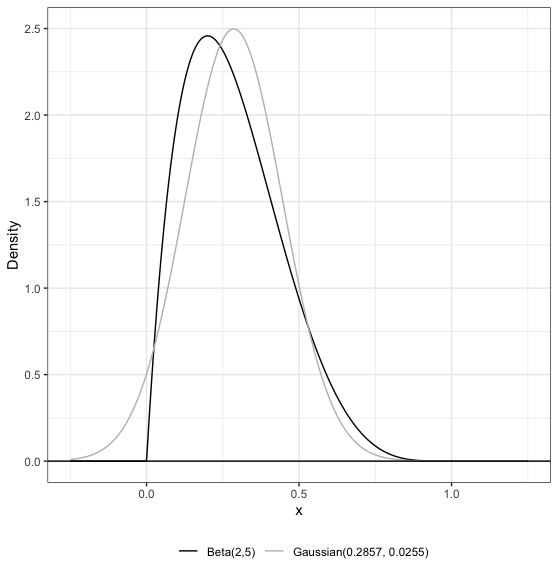
\includegraphics[scale=0.3]{beta distribution with alpha 2 beta 5.png}
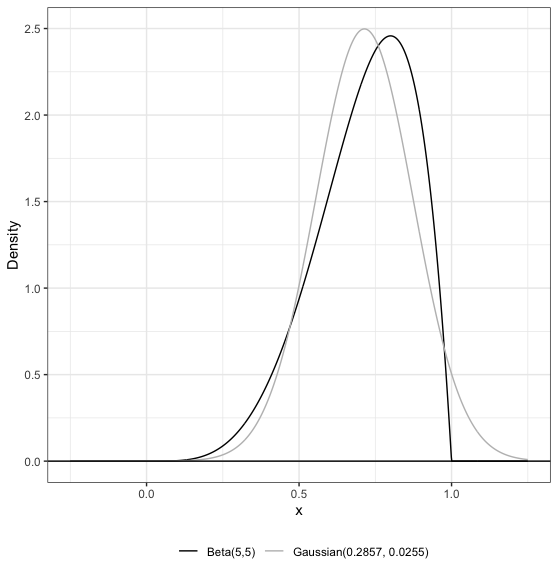
\includegraphics[scale=0.3]{beta distribution with alpha 5 beta 5.png}\\
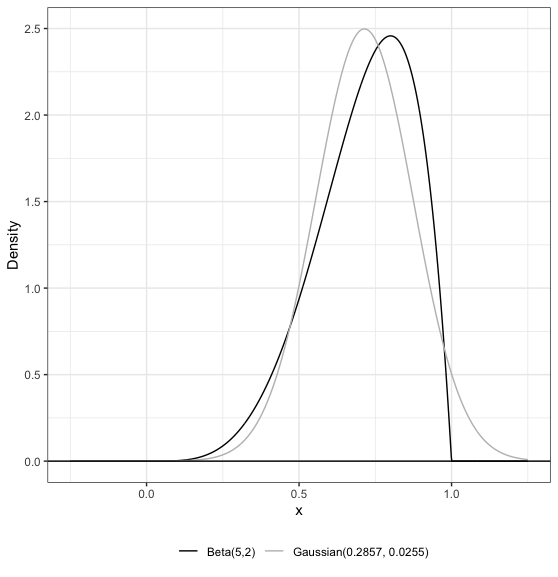
\includegraphics[scale=0.3]{beta distribution with alpha 5 beta 2.png}
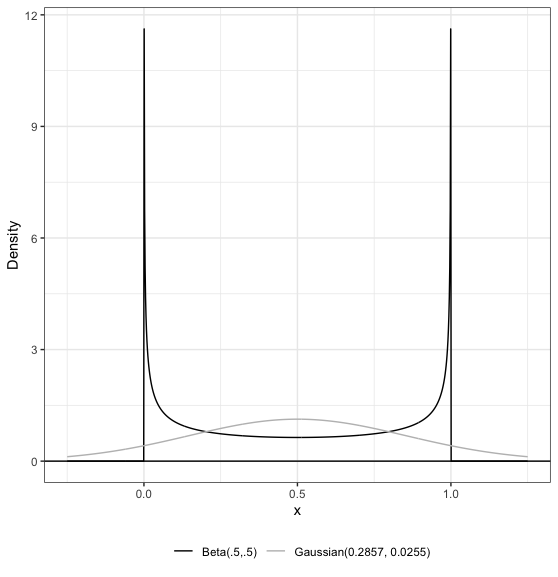
\includegraphics[scale=0.3]{beta distribution with alpha .5 beta .5.png}


\subsection{Population Distribution and Approximation}
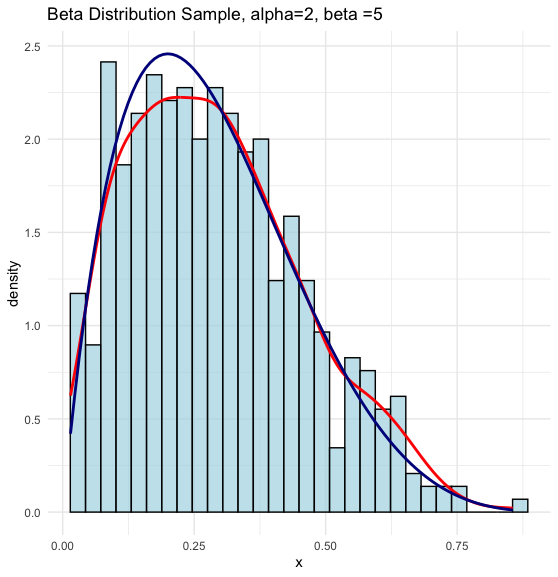
\includegraphics[scale=0.3]{beta distribution alpha 2 beta 5 with sample data.png}
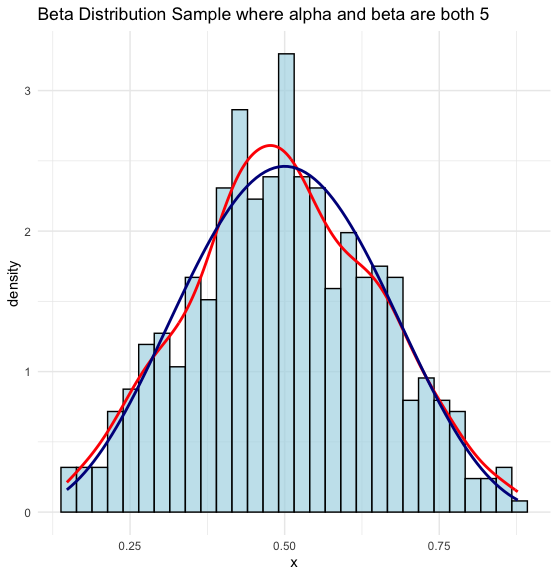
\includegraphics[scale=0.3]{beta distribution with alpha 5 beta 5 with sample data.png}\\
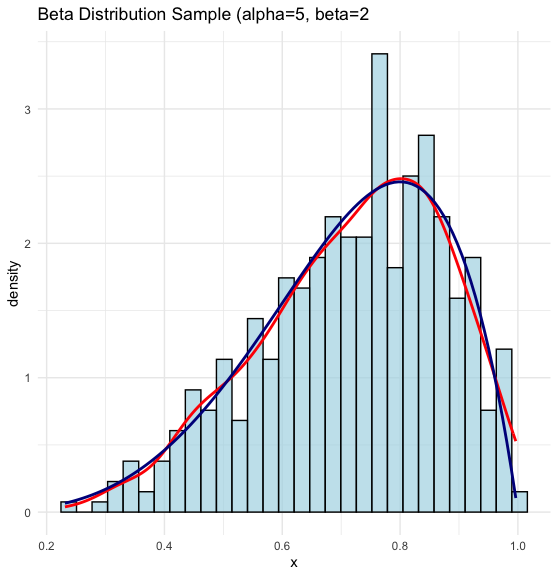
\includegraphics[scale=0.3]{beta distribution with alpha 5 beta 2 with sample data.png}
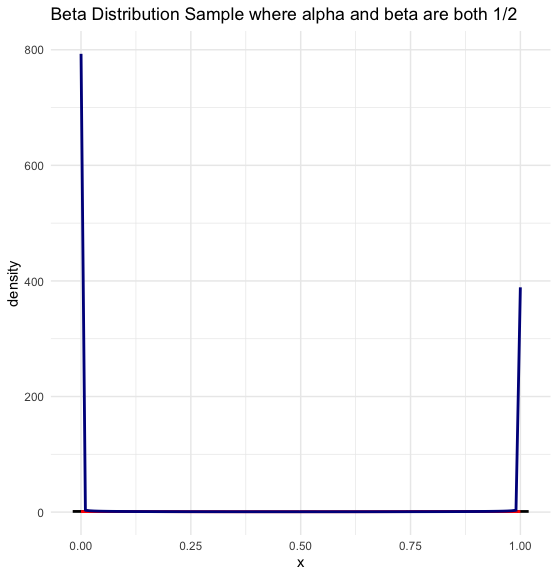
\includegraphics[scale=0.3]{beta distribution with alpha .5 beta .5 with sample data.png}


\subsection{Sample Size and the Beta Distribution}

\includegraphics[scale=0.8]{part 4.png}

\subsection{Modeling Variance with a Sampling Distribution}
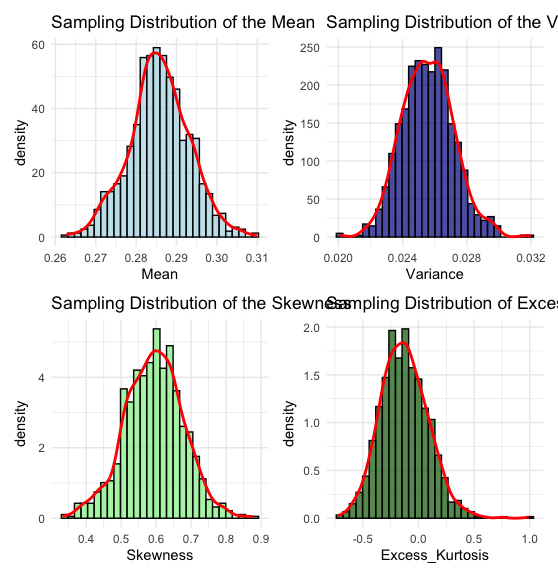
\includegraphics[scale=0.8]{sampling distributions of summary stats (part 5).png}


\subsection{2022 Death Rates Example}
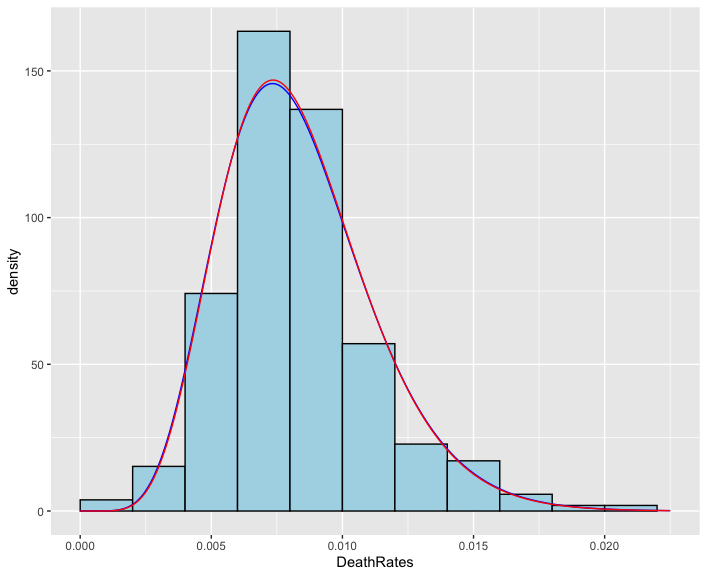
\includegraphics[scale=0.6]{Histogram of Data with distributions super imposed.png}\\
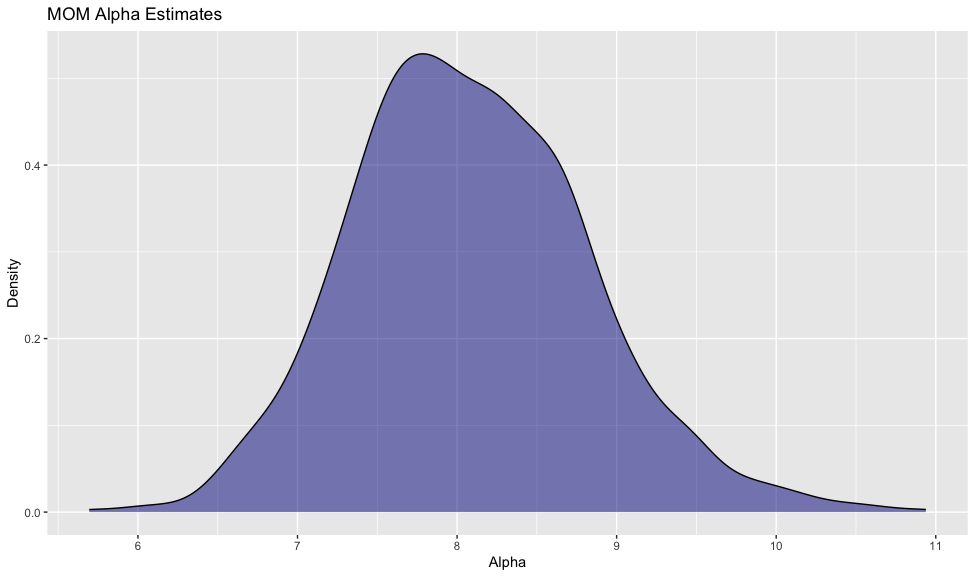
\includegraphics[scale=0.25]{MOM ALPHA DENSITY.png}
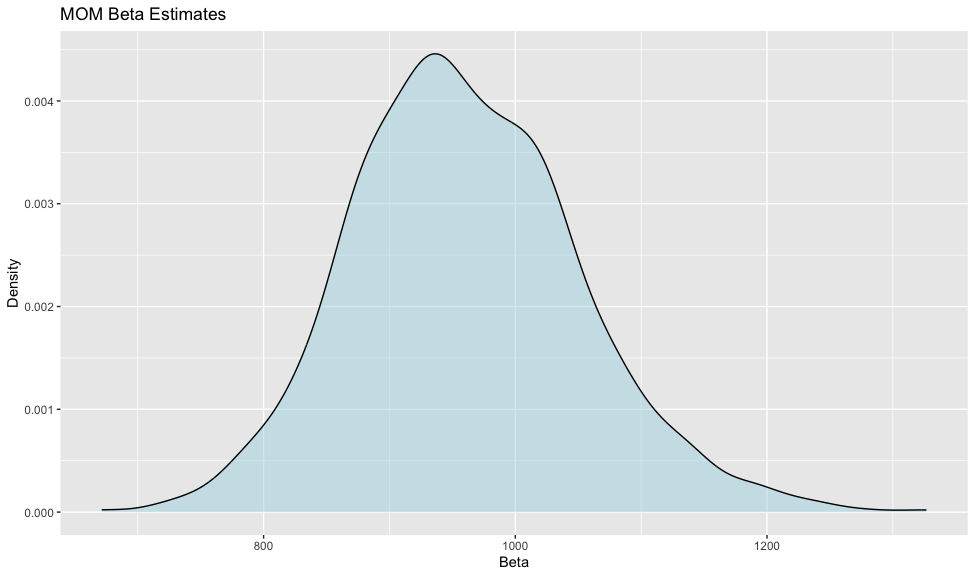
\includegraphics[scale=0.25]{MOM BETA DENSITY.png}\\
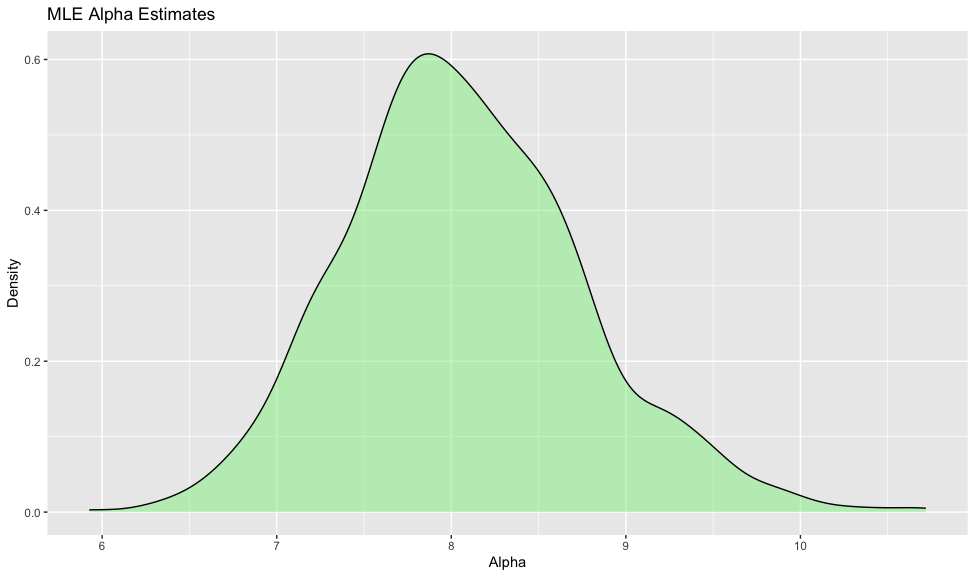
\includegraphics[scale=0.25]{MLE ALPHA DENSITY.png}
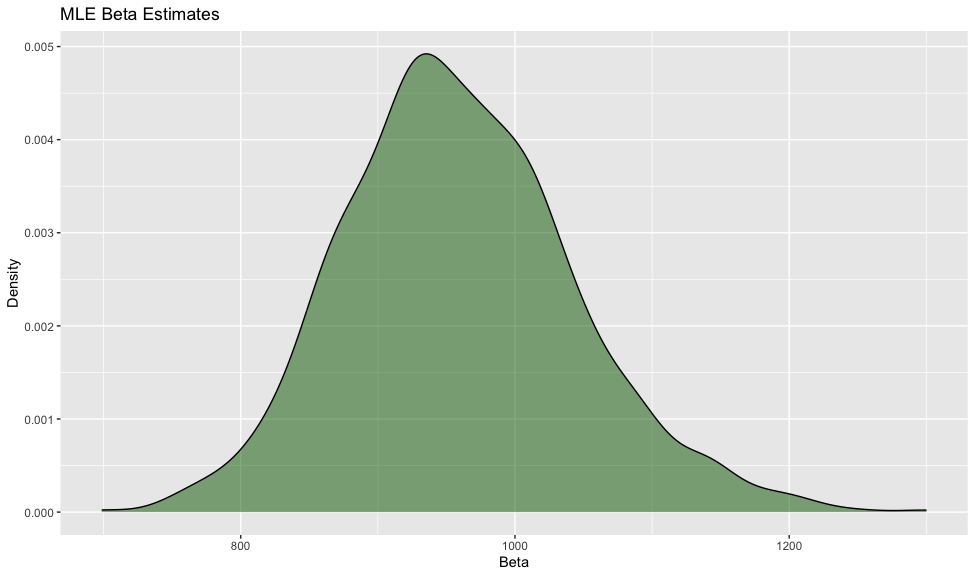
\includegraphics[scale=0.25]{MLE BETA DENSITY.png}





\end{document}
